% --------------
% introduccion
% --------------

La soluci\'on de la ecuaci\'on de Kohn-Sham implica un c\'alculo de muchas 
variables por lo que se usa el m\'etodo autoconsistente. En la soluci\'on de esta ecuaci\'on se usa la expansi\'on en ondas planas y se aproxima el potencial at\'omico con un pseudopotencial e involucra el c\'alculo de integrales en el espacio rec\'iproco. A continuaci\'on se muestra el criterio seguido para cortar el desarrollo de ondas planas y se discuten algunos aspectos relacionados con los m\'etodos computacionales.

% -----------------
% energia de corte
% -----------------

\section{Energ\'ia de corte}
La expansi\'on en ondas planas puede contener un n\'umero infinito de t\'erminos haciendo dif\'icil su manejo computacional. Para reducir el n\'umero de ondas planas se define una energ\'ia de corte $E_{cut}$

\begin{equation}
    E_{cut} \ge \frac{1}{2} |K + G|^{2}  \textup{ ,}
\end{equation}

\noindent todas las ondas planas por debajo de este limite son tomadas en cuenta en la expansi\'on. Una forma esquematica de ver esta energ\'ia de corte se observa en la figura \ref{EnergiaCorte}.


\begin{figure}[H]
    \centering
    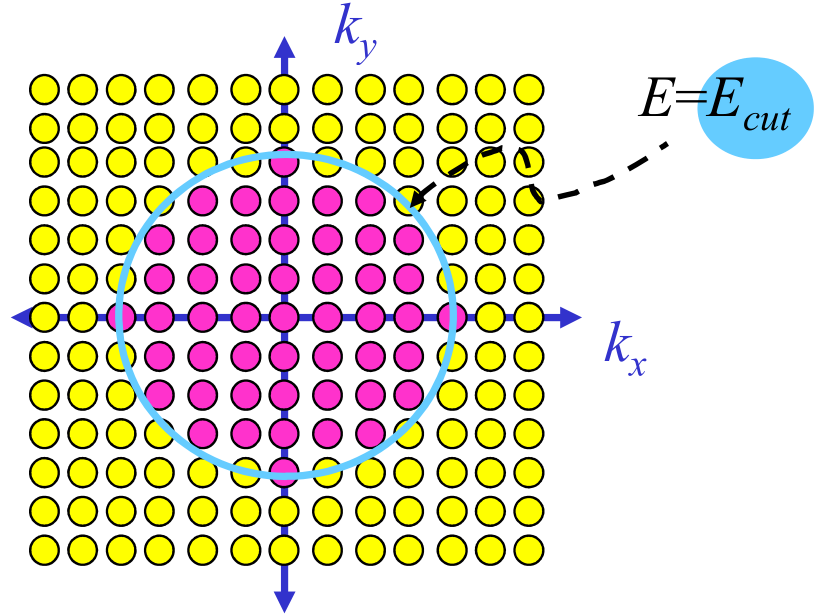
\includegraphics[width=0.6\linewidth]{contenido/calculos_computacionales/energia_corte/img_corte/EnergiaCorte}
    \caption{Representaci\'on esquem\'atica de la energ\'ia de corte.}
    \label{EnergiaCorte}
\end{figure}

\noindent La energ\'ia de corte es un par\'ametro que debe ser calculado espec\'ificamente para cada sistema tratado.

% -----------------
% Pseudopotencial
% -----------------

\section{Pseudopotencial}
Dentro del \'atomo podemos distinguir tres componentes: el n\'ucleo at\'omico, los electrones centrales 
y los electrones de valencia (figura \ref{ElectronSeparation}). Los electrones centrales se ubican en las 
capas m\'as cercanas al n\'ucleo  y sus estados  no se ven alterados por la presencia de otros \'atomos, 
es decir se comportan como si fueran inertes. Por el contrario, los electrones de valencia se encuentran 
en las capas m\'as externa del \'atomo y son los responsables del enlace entre los \'atomos. La 
aproximaci\'on del pseudopotencial se basa en estas distinciones entre electrones.

\begin{figure}[H]
    \centering
    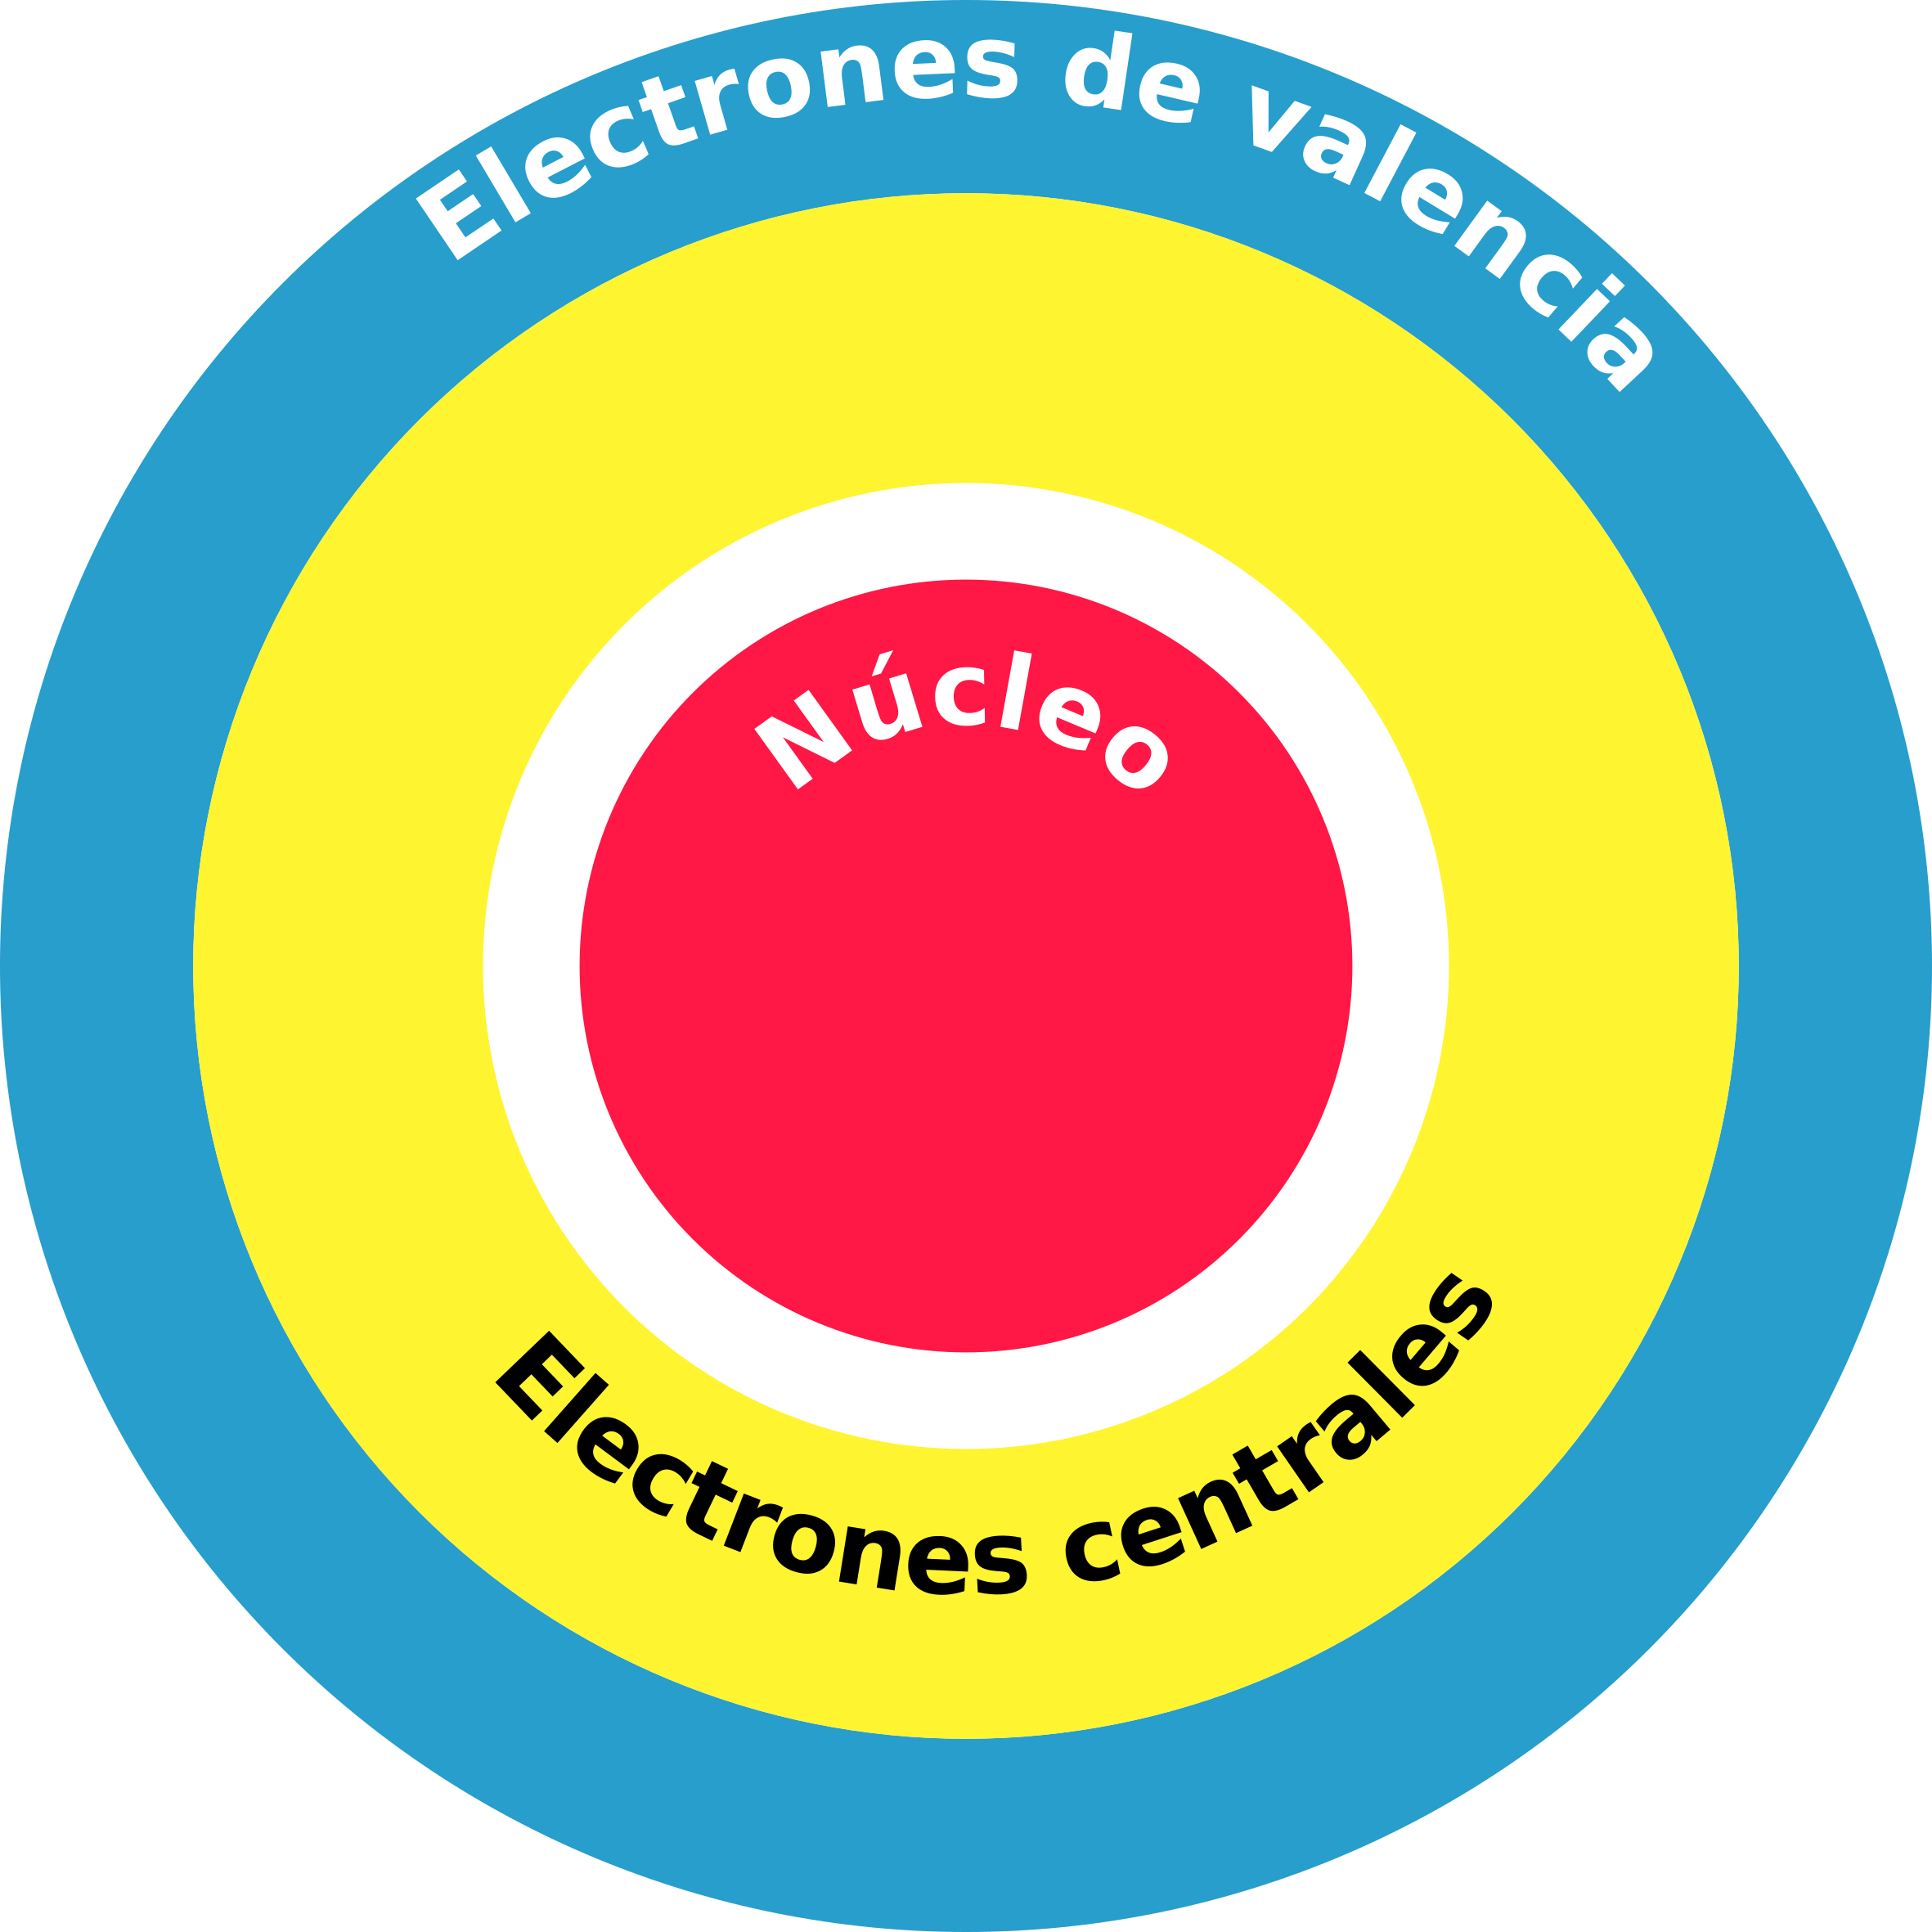
\includegraphics[width=0.3\textwidth]{contenido/calculos_computacionales/pseudopotencial/img_pseudopotencial/electrons_separation.png}
    \caption[Representaci\'on esquem\'atica de los electrones 
    centrales y de 
    valencia]{Representaci\'on esquem\'atica de los electrones 
    centrales y de 
    valencia.}
    \label{ElectronSeparation}
\end{figure}

\noindent La funci\'on de onda de los electrones de valencia oscila 
r\'apidamente (figura 
\ref{pseudopotential}), cuando 
atraviesa la secci\'on de los electrones centrales dado que estos 
deben 
mantenerse ortogonales entre ellos y hace muy dif\'icil su soluci\'on 
num\'erica. 

\begin{figure}[H]
    \centering
    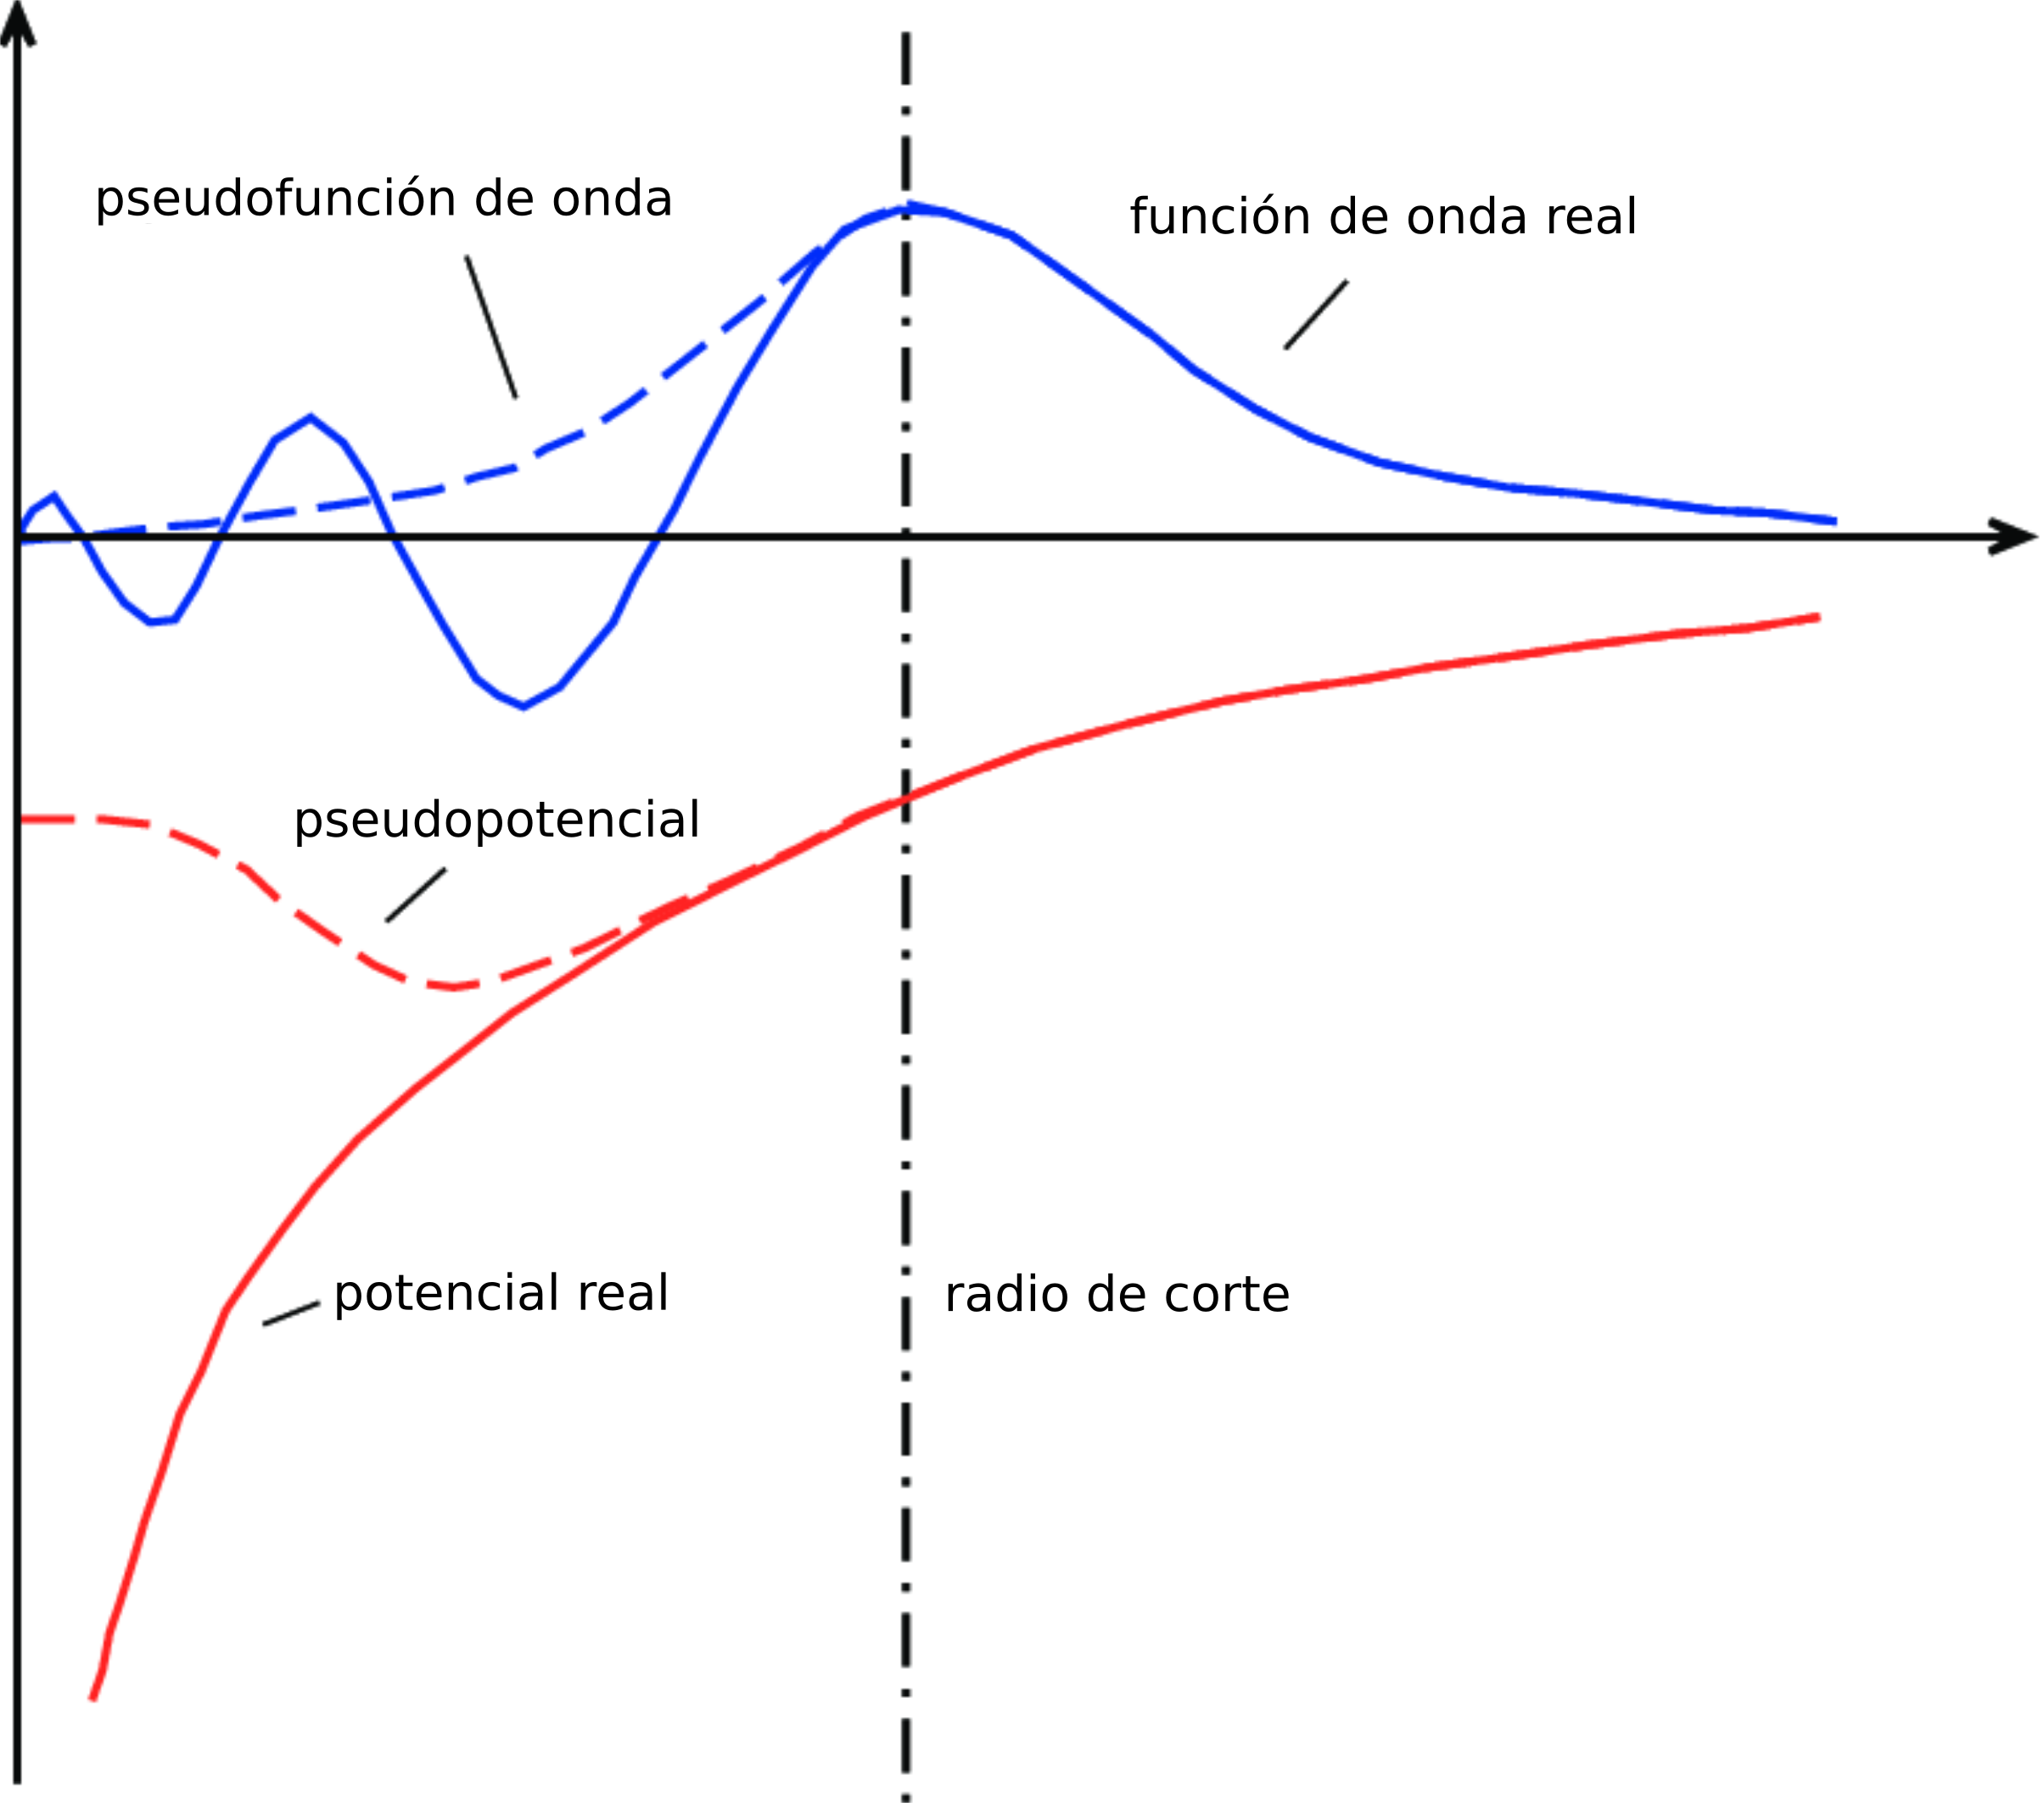
\includegraphics[width=0.4\textwidth]{contenido/calculos_computacionales/pseudopotencial/img_pseudopotencial/pseudopotential.png}
    \caption[Representaci\'on esquem\'atica del potencial real y del 
    pseudopotencial]{Representaci\'on esquem\'atica del potencial real y del 
    pseudopotencial.}
    \label{pseudopotential}
\end{figure}

\noindent La aproximaci\'on de los pseudopotenciales, reemplaza estas funciones 
de 
valencia por pseudofunciones de valencia que desempe\~nan el mismo rol 
que las 
originales pero evitando el comportamiento nodal cerca del n\'ucleo. 
Esto se 
logra considerando un pseudopotencial m\'as suave que el potencial del 
n\'ucleo 
original (figura \ref{pseudopotential}), debido a que se consideran a 
los 
electrones centrales y al n\'ucleo como una sola entidad que da origen 
al 
pseudopotencial (figura \ref{ElectronUnion}).

\begin{figure}[H]
    \centering
    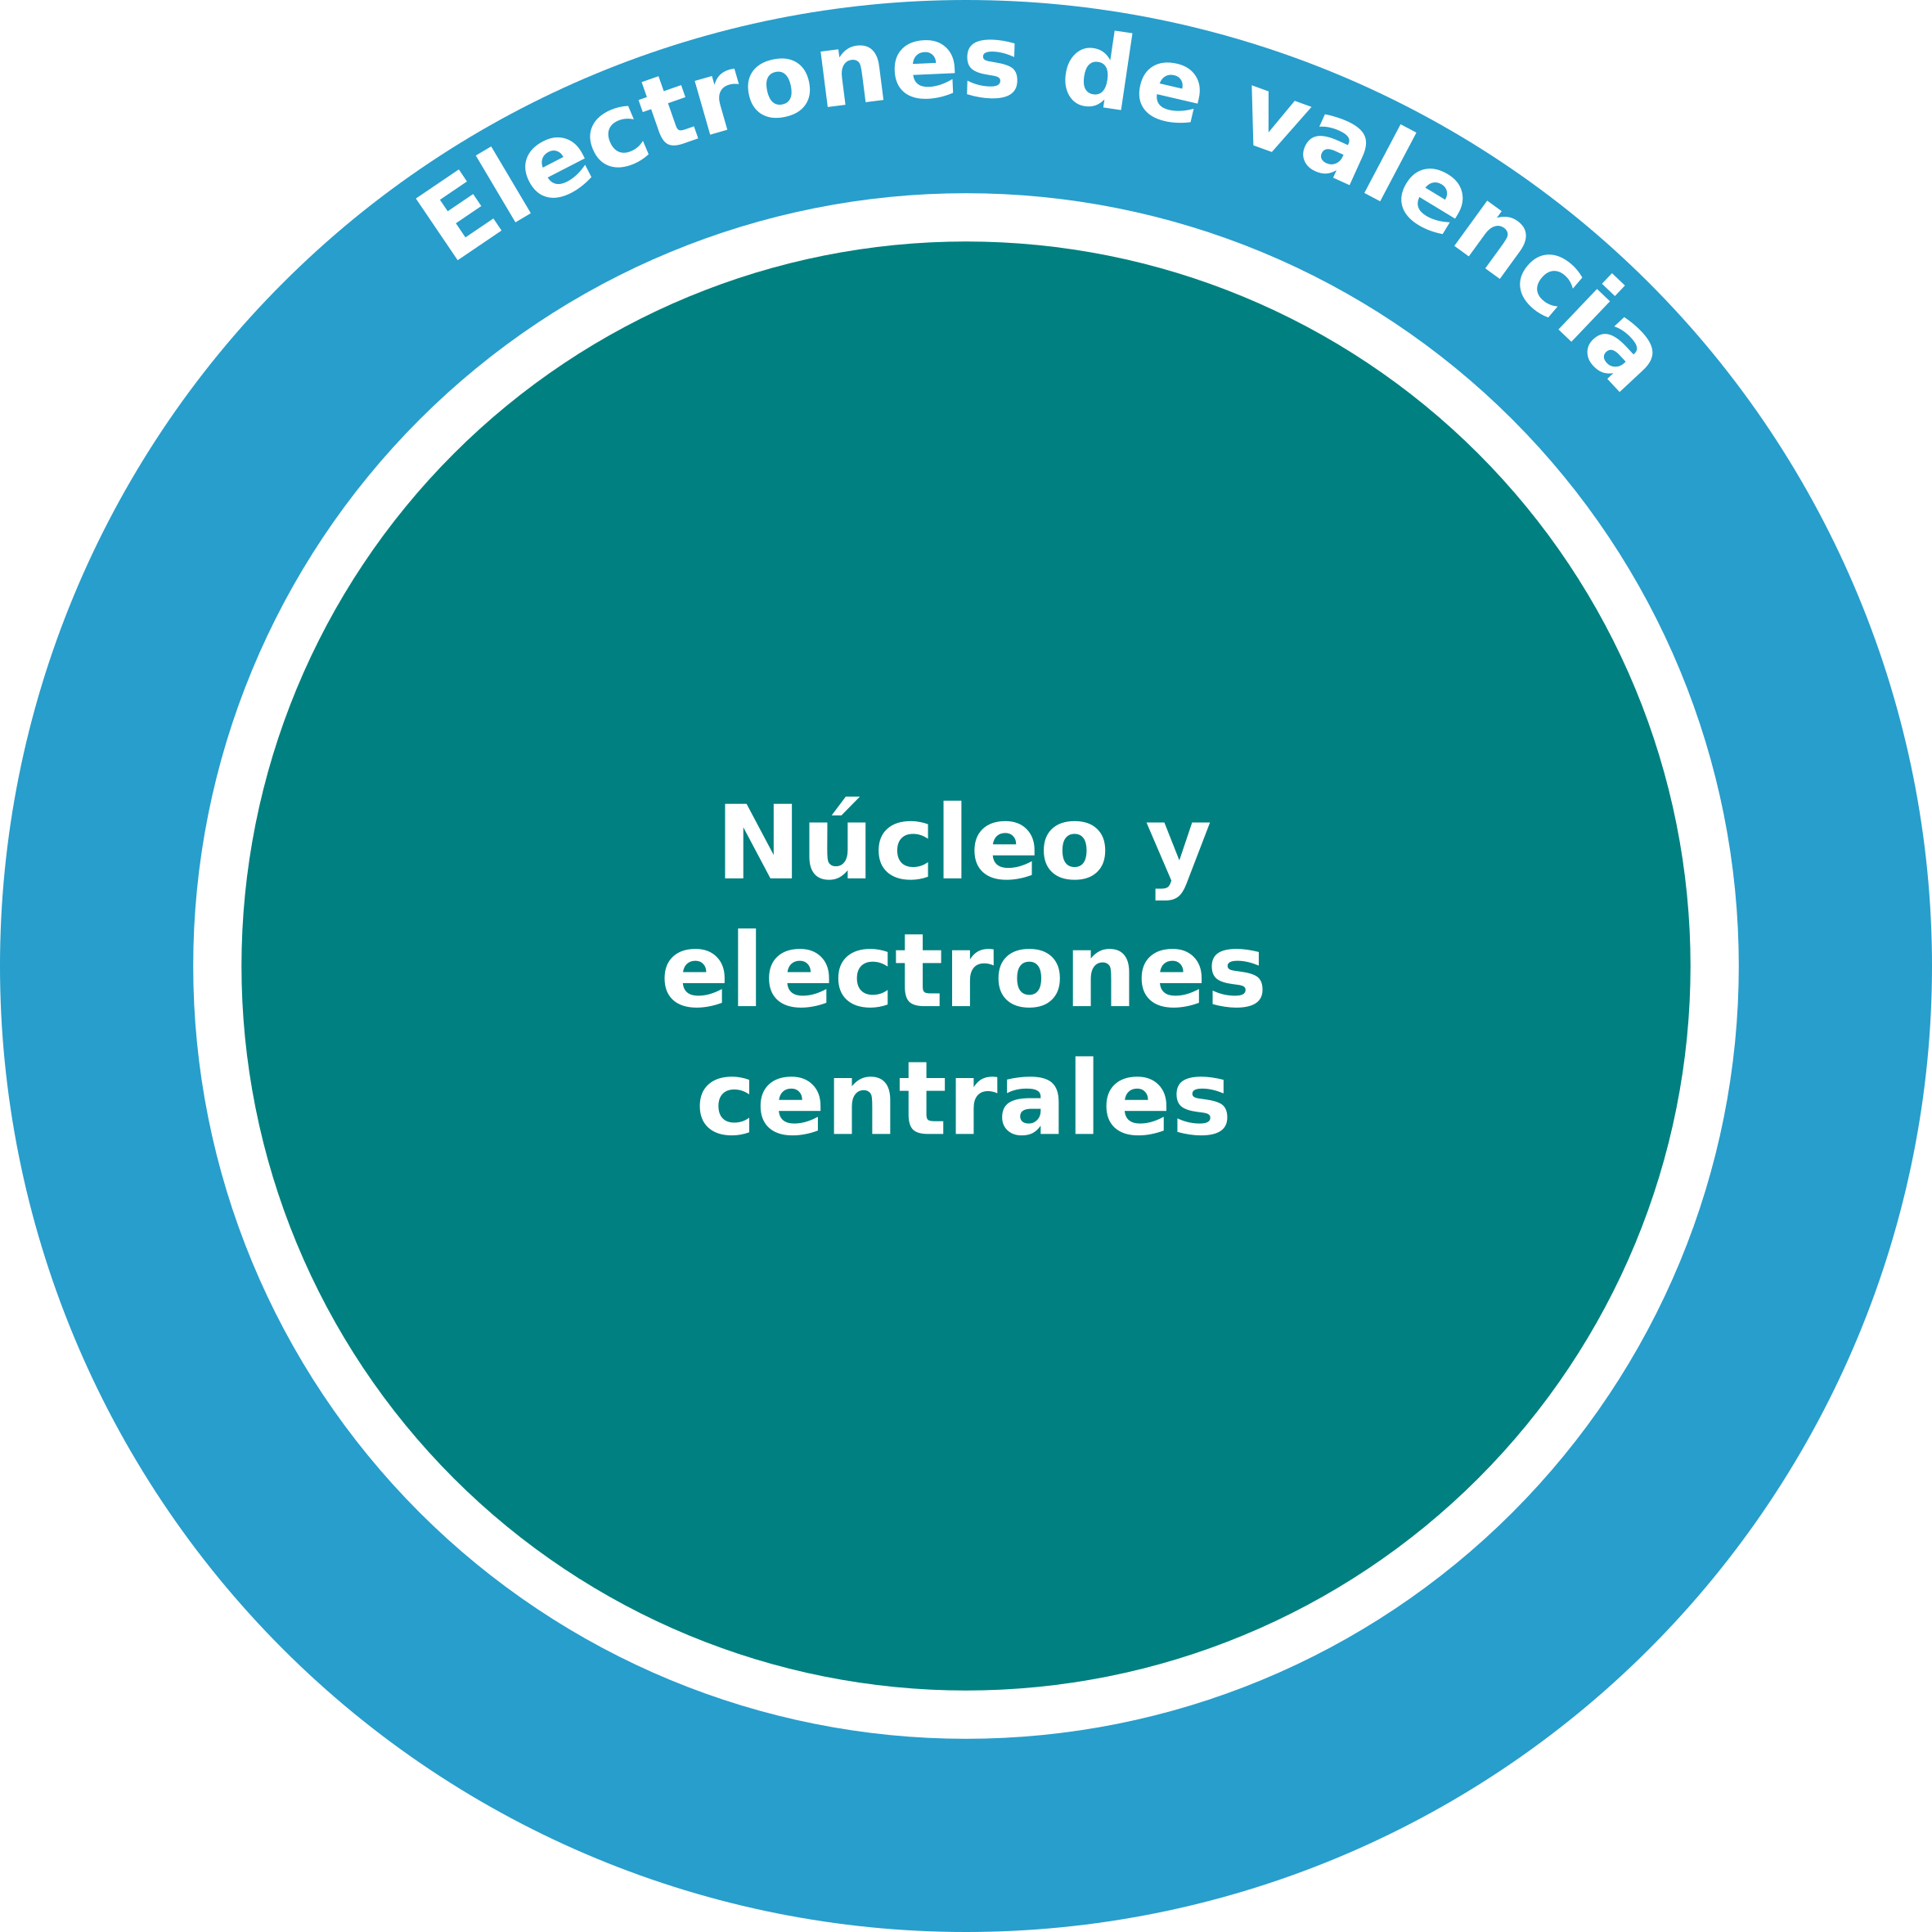
\includegraphics[width=0.3\textwidth]{contenido/calculos_computacionales/pseudopotencial/img_pseudopotencial/ElectronUnion.png}
    \caption[Representaci\'on esquem\'atica de la aproximaci\'on del 
    n\'ucleo 
    con los electrones centrales]{Representaci\'on esquem\'atica de la 
    aproximaci\'on del 
    n\'ucleo 
    con los electrones centrales.}
    \label{ElectronUnion}
\end{figure}

\noindent Las propiedades de dispersi\'on de cualquier pseudopotencial deben 
ser 
id\'enticas a las propiedades de dispersi\'on del potencial i\'onico 
real. Esto 
es necesario para que el pseudopotencial sea considerado \'util, adem\'as el 
pseudopotencial debe ser transferible es decir que debe ser valido para 
cualquier 
estructura cristalina o s\'olido en el que sea introducido el \'atomo al 
que 
pertenece el pseudopotencial.

% -----------------
% integrales espacio reciproco
% -----------------

\section{Integrales en el espacio rec\'iproco}
Cantidades como la densidad de estados, la densidad de carga entre otras requieren de integrales sobre el espacio rec\'iproco.

\begin{equation}
    \bar{A} = \int _{BZ} A(k) d(k)
\end{equation}

\noindent Para que la integral sea evaluada computacionalmente debe ser discretizada mediante una sumatoria de pesos que se asignan a los puntos del espacio rec\'iproco.

\begin{equation}
    \int _{BZ} d(k) \to \sum _{K} w_{K}
\end{equation}

\noindent A continuaci\'on se da un ejemplo con una grilla de $4 \times 4$.

\begin{figure}[H]
    \centering
    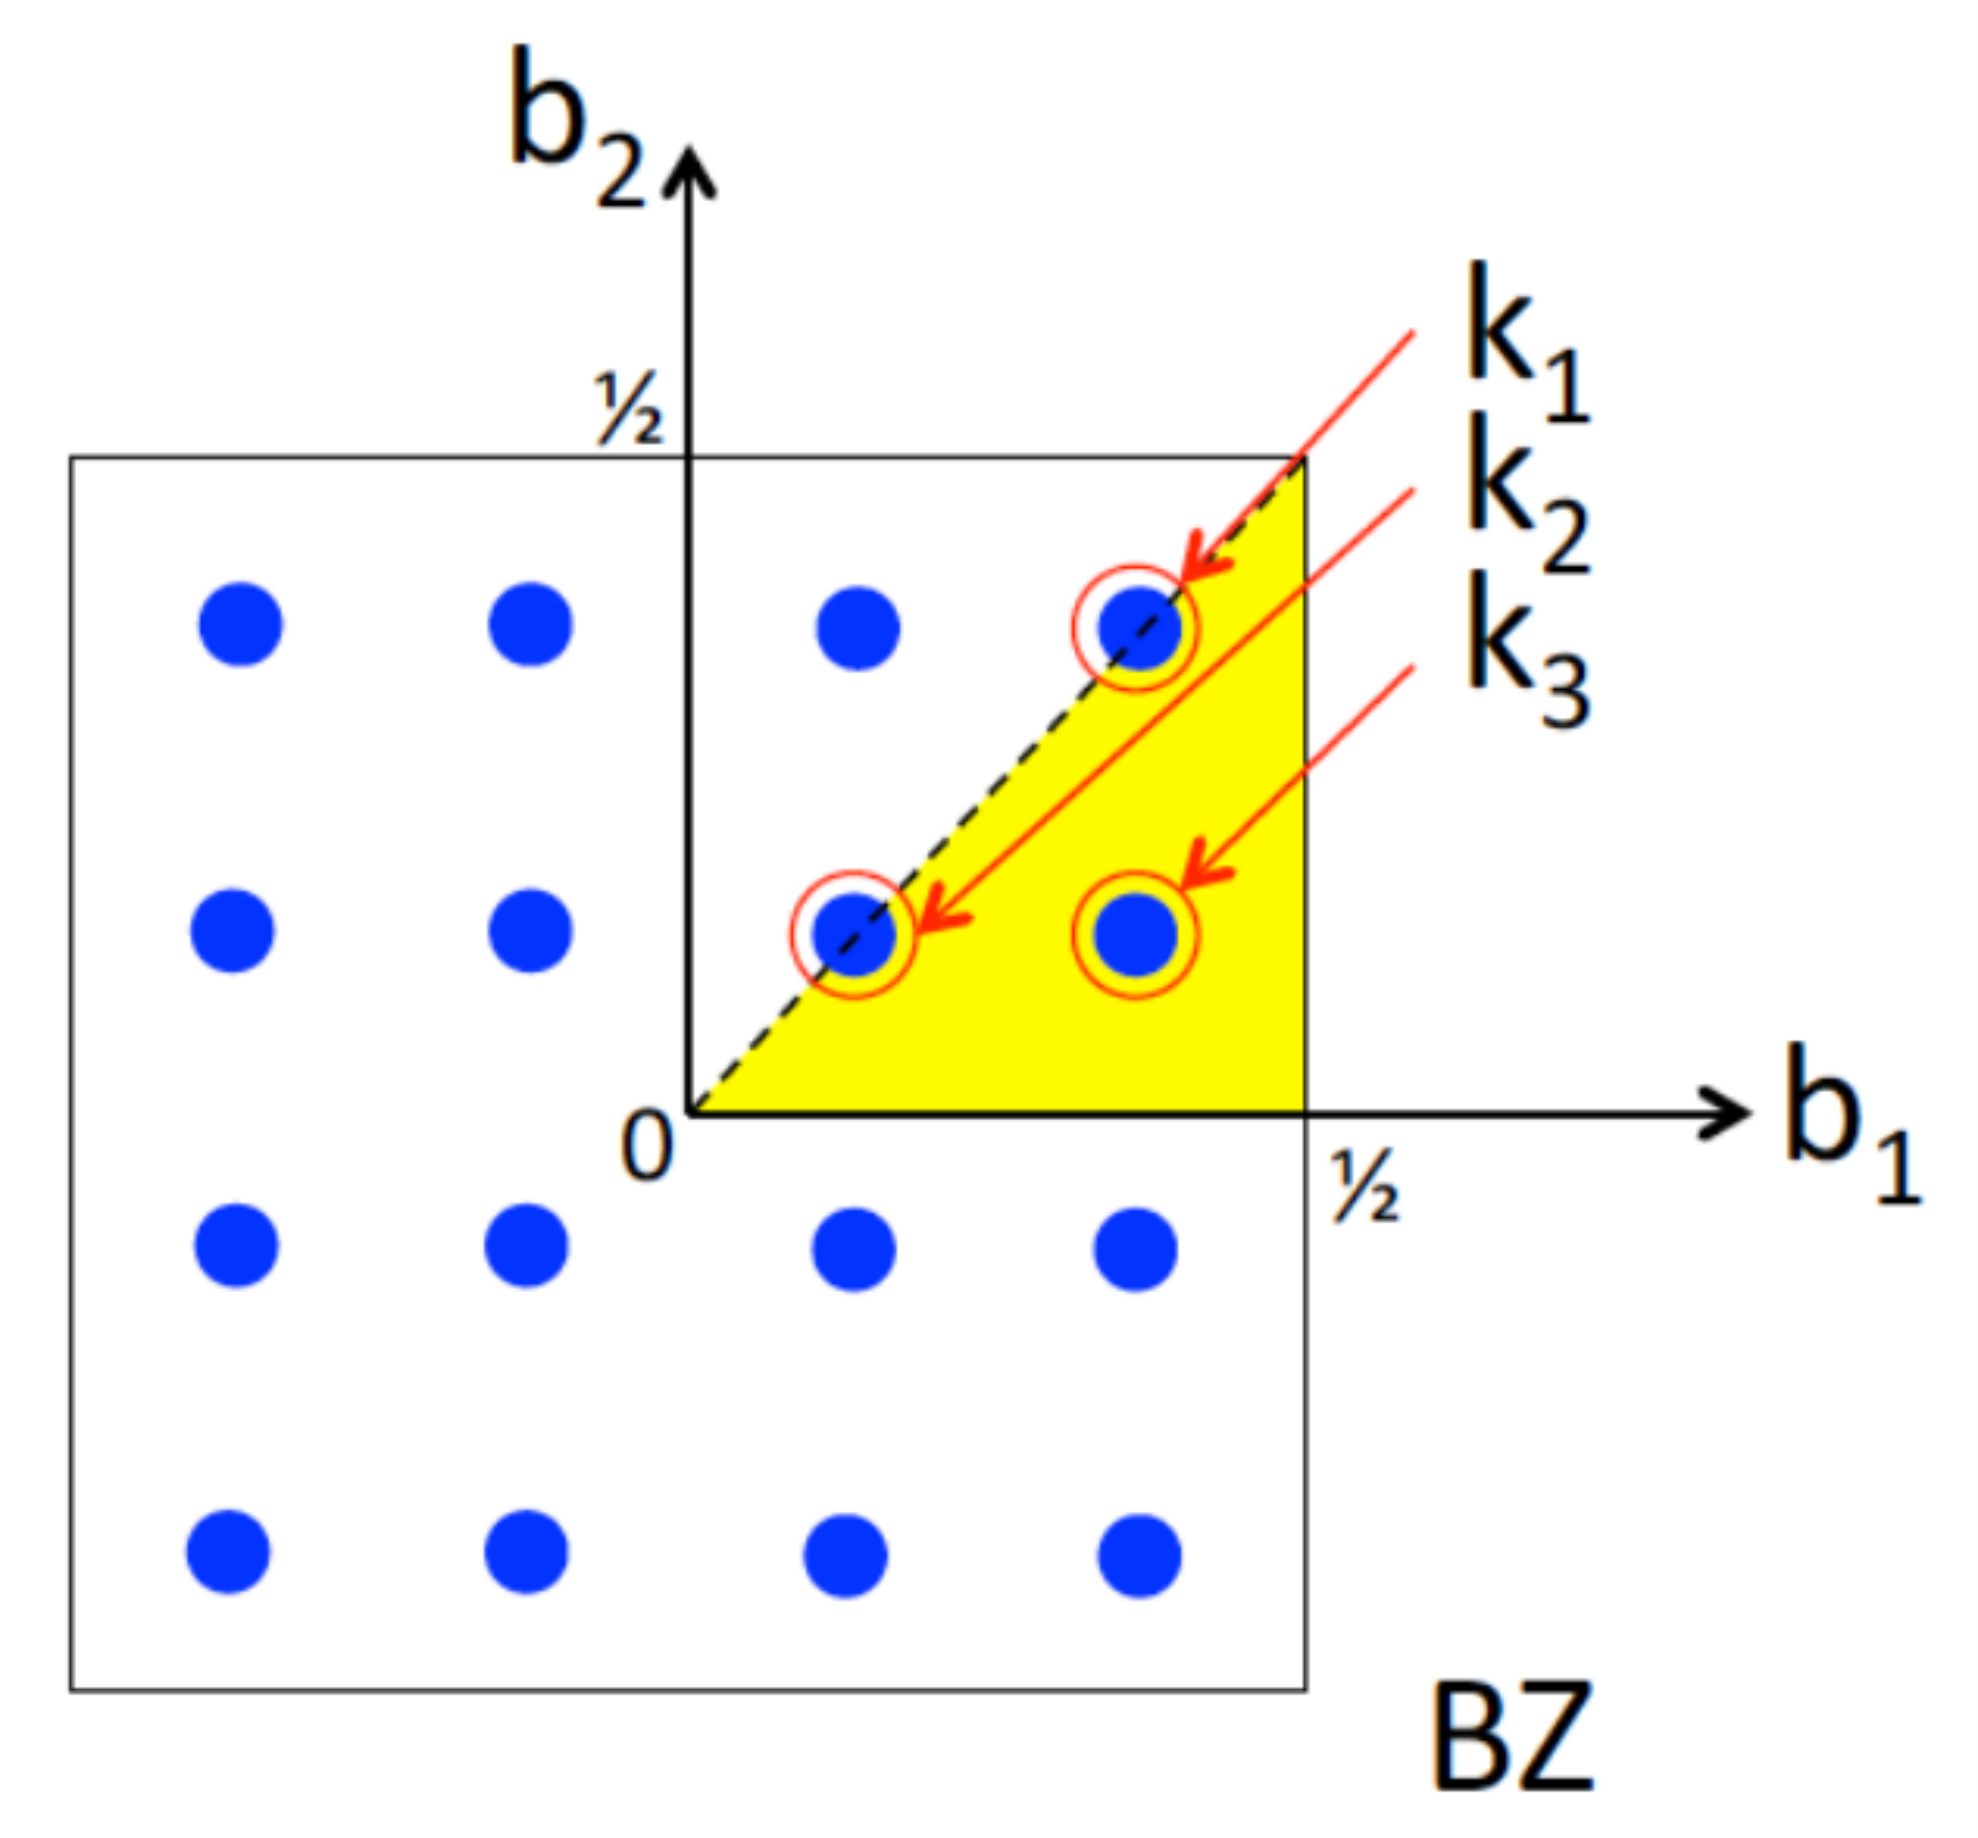
\includegraphics[width=0.6\linewidth]{contenido/calculos_computacionales/integrales_reciproco/img_reciproco/ZonaBrillouin}
\end{figure}

\noindent los pesos correspondientes son los siguientes.

\begin{eqnarray}
4 \times K_{1} \to w_{1} = \frac{4}{16} = \frac{1}{4} \nonumber \\
4 \times K_{2} \to w_{2} = \frac{4}{16} = \frac{1}{4}  \\
8 \times K_{3} \to w_{1} = \frac{8}{16} = \frac{1}{2} \nonumber
\end{eqnarray}

\noindent la integral discretizada seria la siguiente

\begin{equation}
    \int _{BZ} A(k) d(k) \approx \frac{1}{4}A(K_{1}) + \frac{1}{4}A(K_{2}) + \frac{1}{2}A(K_{3})
\end{equation}


% -----------------
% calculo de U hubbard
% -----------------

\section{C\'alculo del potencial U de Hubbard}
El valor del par\'ametro U de Hubbard debe ser calculado para cada material estudiado. Un posible m\'etodo es el semiemp\'irico que consiste en probar varios valores del par\'ametro U hasta ajustar los resultados a datos experimentales del material. 
Un m\'etodo m\'as preciso para calcular el par\'ametro U de Hubbard es el m\'etodo de respuesta lineal, el cual se describe a continuaci\'on y fue el m\'etodo usado en este trabajo.

\subsection{M\'etodo de respuesta lineal}

El m\'etodo de respuesta lineal fue propuesto por Cococcioni y Gironcoli en el a\~no 2005 \cite{cococcioni2005}. Este m\'etodo consiste en realizar peque\~nas perturbaciones en la energ\'ia de los orbitales {\bf d}. Para medir la respuesta del sistema a las perturbaciones el m\'etodo propone estudiar el cambio de las ocupaciones de los orbitales {\bf d} respecto a las perturbaciones. En el m\'etodo el par\'ametro U se expresa de la siguiente forma.

\begin{equation}
    U = \chi _{0}^{-1} - \chi ^{-1} \textup{ ,}
\end{equation}

\noindent que toma en cuenta la energ\'ia asociada al cambio de una poblaci\'on de electrones y la energ\'ia asociada al cambio en otro estado, donde $\chi_{0}$ y $\chi$ se definen como

\begin{equation}
    \chi = \frac{dn}{d\alpha}
    \label{definicion_chi}
\end{equation}

\noindent Las perturbaciones deben ser peque\~nas y los valores tomados se encuentran normalmente alrededor de cero. Esto se aplicara a los electrones en estado {\bf d} ya que se espera un cambio de energ\'ia significativo por estar alejados del n\'ucleo.

\noindent Para utilizar este m\'etodo con Quantum ESPRESSO, se deben seguir los siguientes pasos. Primero se realiza un c\'alculo autoconsistente sin ning\'un tipo de perturbaci\'on, cuya soluci\'on autoconsistente ser\'a tomada como punto de partida para los siguientes c\'alculos. Luego se realizan c\'alculos autoconsistentes separados para cada valor de $\alpha $ considerado. En cada uno de estos c\'alculos se debe guardar el valor de la ocupaci\'on en la primera iteraci\'on y en la \'ultima iteraci\'on cuando alcanza la convergencia, lo cual son resultados accesibles en el programa.
Si graficamos las ocupaciones respecto de las perturbaciones obtenemos una gr\'afica como la siguiente \ref{RespuestaLineal}.


\begin{figure}[H]
    \centering
    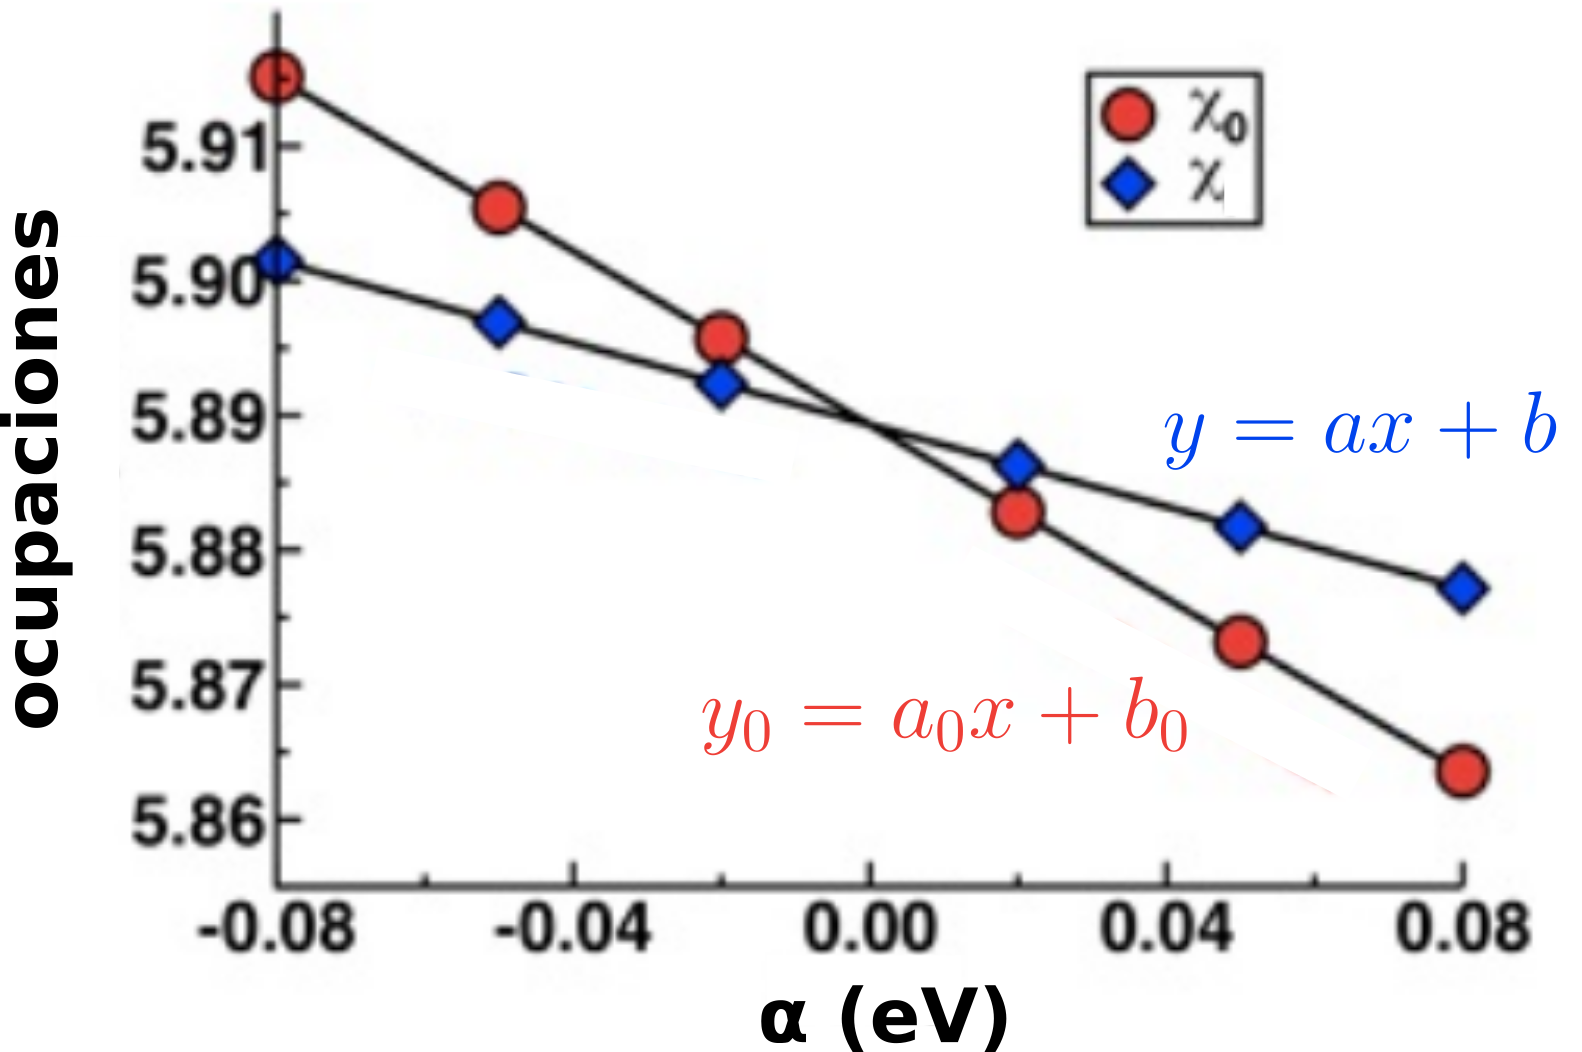
\includegraphics[width=0.6\linewidth]{contenido/calculos_computacionales/calculo_hubbard/img_lineal/RespuestaLineal}
    \caption{Ocupaciones versus perturbaciones.}
    \label{RespuestaLineal}
\end{figure}

\noindent La derivada \ref{definicion_chi} da el valor de $\chi_{0}$ y $\chi$ debe ser evaluada num\'ericamente, en este caso su valor es la pendiente de la recta correspondiente a $\chi_{0}$ o $\chi$. Refiri\'endonos  a la gr\'afica \ref{RespuestaLineal} el valor de $\chi_{0}$ es la pendiente de la recta de puntos rojos y el valor de $\chi$ es la pendiente de la recta de puntos azules.

% --------------------------
% software de uso frecuente
% --------------------------

\section{Softwares de uso frecuente}
Existen muchos paquetes de simulaci\'on que implementan la teor\'ia del 
funcional de densidad. Estos paquetes de simulaci\'on se diferencian por el 
conjunto de funciones base que utilizan, los tipos de pseupotenciales que 
admiten y las propiedades que pueden calcular, entre otros aspectos. A 
continuaci\'on se presenta una lista de algunos paquetes de simulaci\'on 
relevantes.

\begin{itemize}
    \item \textbf{VASP:}  Es un paquete de simulaci\'on para modelamiento de 
    materiales a escala at\'omica como c\'alculos de estructura electr\'onica y 
    din\'amica molecular mec\'anico-cu\'antica a partir de primeros principios. 
    Implementa la teor\'ia del funcional de densidad, funcionales h\'ibridos, 
    teor\'ia de perturbaci\'on y el m\'etodo de funciones de Green. Adem\'as 
    utiliza pseudopotenciales, m\'etodo del proyector de ondas aumentadas y 
    ondas planas.
    \item \textbf{WIEN2k:} Es un paquete de simulaci\'on que permite realizar 
    c\'alculos de estructura electr\'onica de s\'olidos usando la teor\'ia del 
    funcional de densidad. Implementa el m\'etodo de ondas planas aumentadas 
    linealizadas m\'as orbitales locales (LAPW + lo) y tambi\'en es capaz de 
    considerar efectos relativistas.
    \item \textbf{ABINIT:} Es un paquete de simulaci\'on para c\'alculos de 
    estructura electr\'onica que implementa la teor\'ia del funcional de 
    densidad con pseudopotenciales o wavelets. Adem\'as implementa la teor\'ia 
    de perturbaciones y la teor\'ia del funcional de densidad dependiente del 
    tiempo.
    \item \textbf{Quantum ESPRESSO:} Es una suite de paquetes de simulaci\'on 
    para c\'alculos de estructura electr\'onica que implementa la teor\'ia del 
    funcional de densidad utilizando pseudopotenciales y ondas planas. Adem\'as 
    implementa la teor\'ia del funcional de densidad dependiente del tiempo. 
    Este es el software que se utiliza en el presente estudio.
\end{itemize}

% -----------------------
% suite quantum espresso
% -----------------------

\section[C\'alculos de estructura electr\'onica usando la suite Quantum \\
ESPRESSO]{C\'alculos de estructura electr\'onica usando la suite Quantum 
	ESPRESSO}
El siguiente diagrama muestra el proceso que se sigue en un c\'alculo autoconsistente convencional con Quantum ESPRESSO.

\begin{figure}[H]
	\centering
	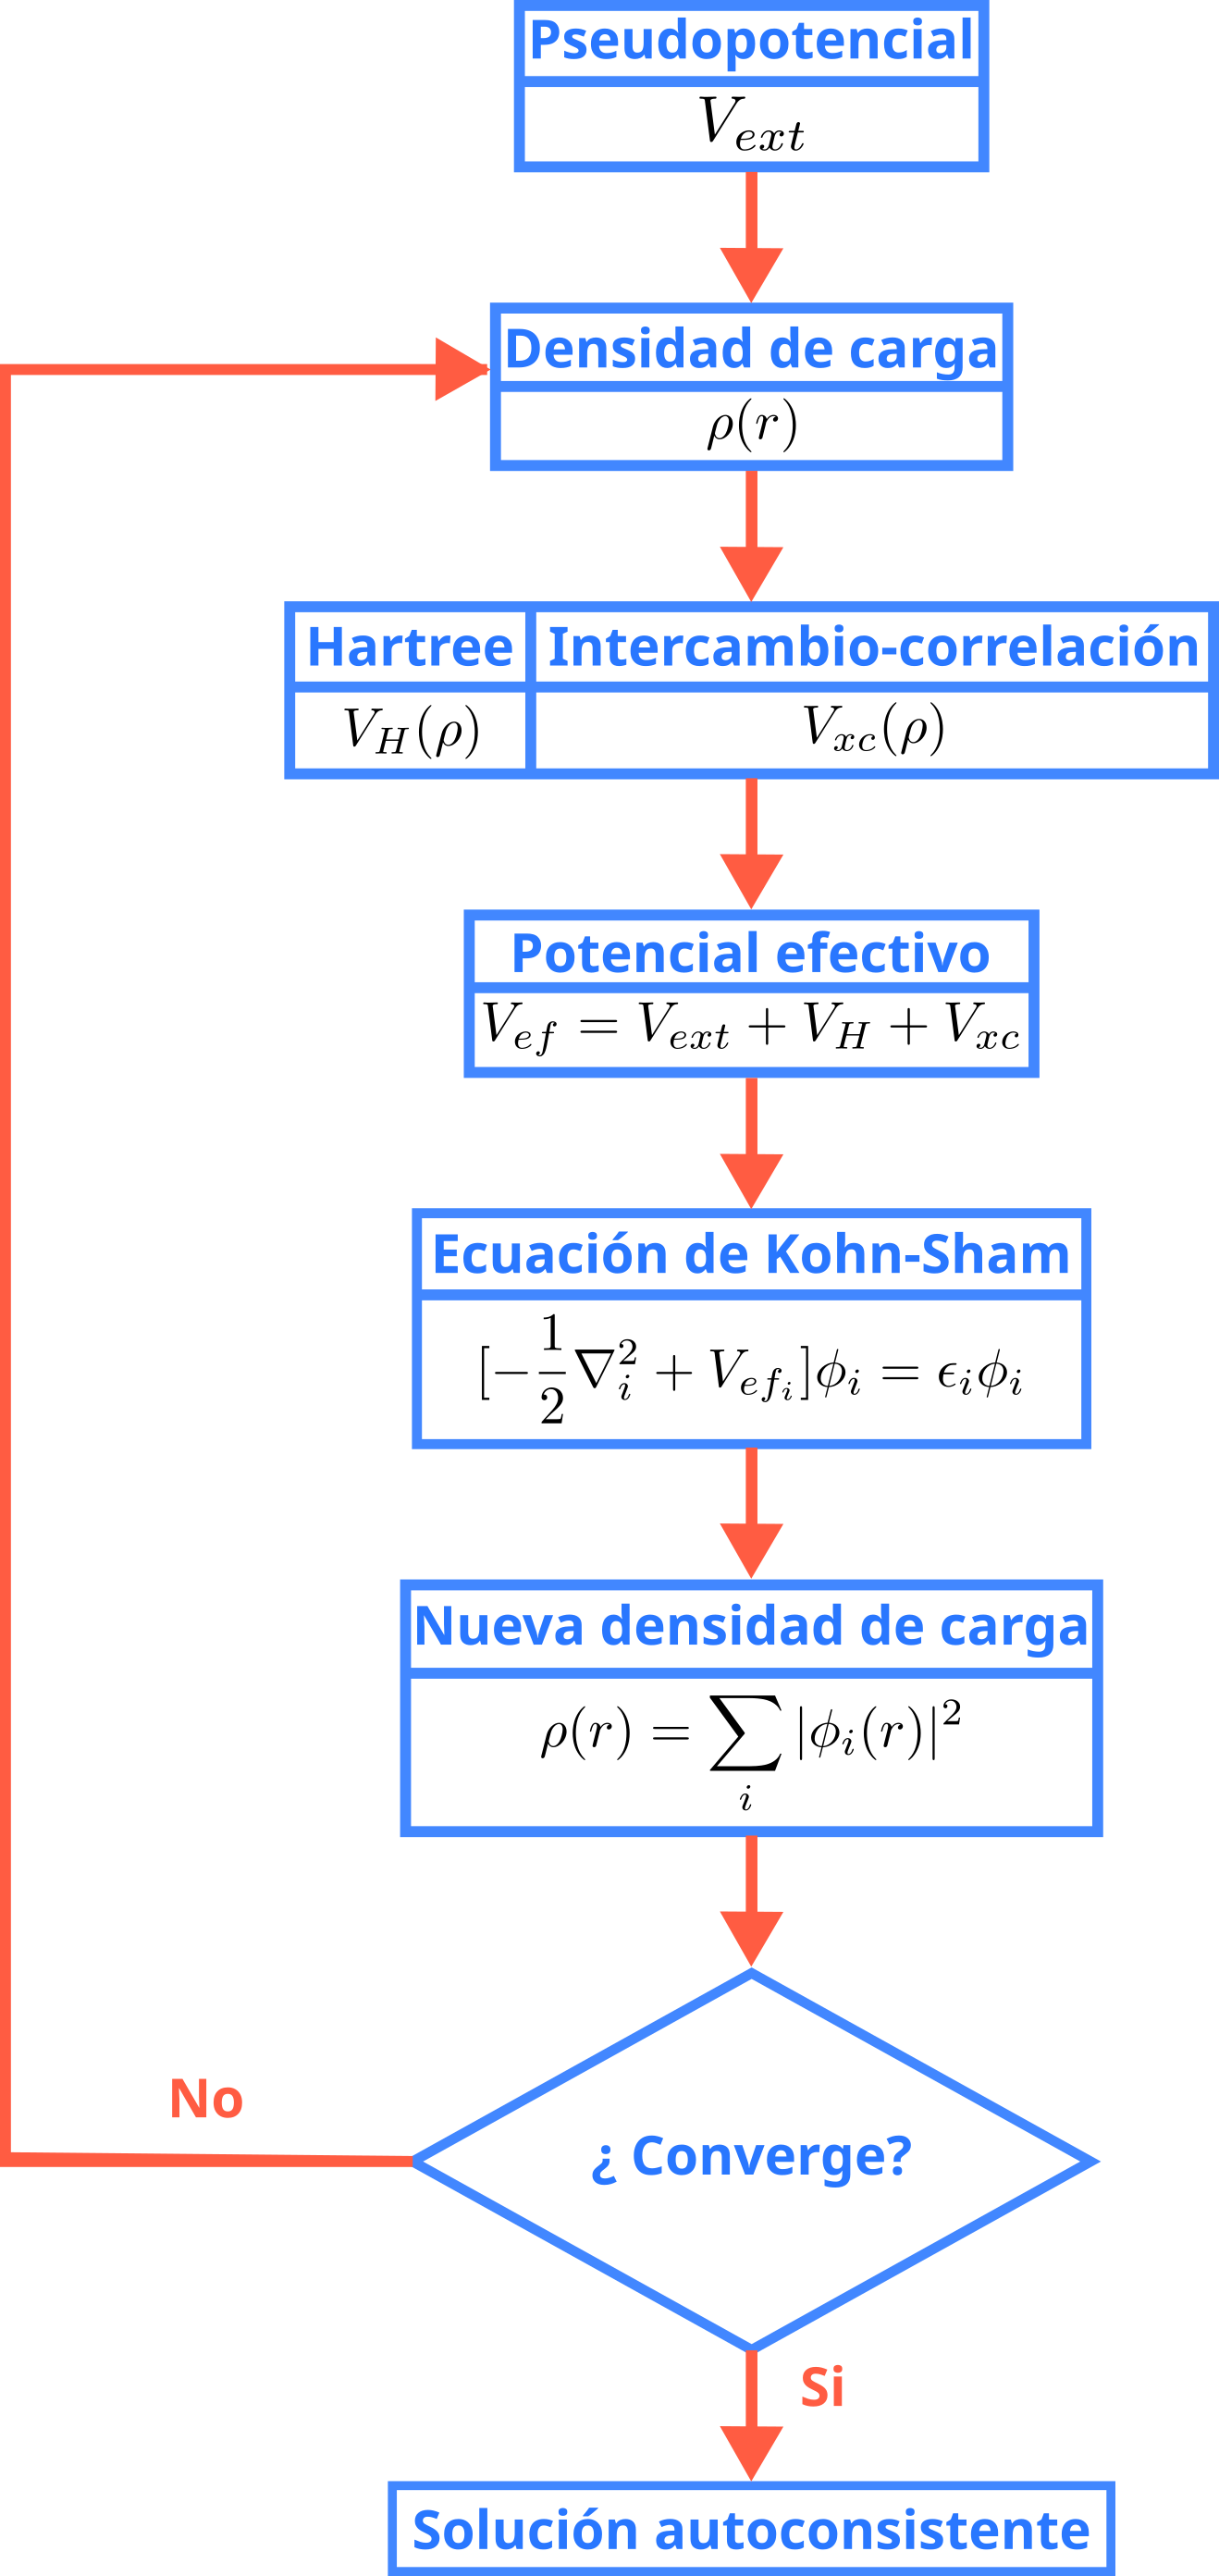
\includegraphics[width=0.4\textwidth]{contenido/calculos_computacionales/suite_qe/img_suite_qe/BucleAutoconsistente.png}
	\caption[Diagrama del proceso de c\'alculo de campo 
	autoconsistente]{Diagrama del proceso de c\'alculo de campo 
		autoconsistente.}
\end{figure}

Quantum ESPRESSO se encuentra formado por varios programas que cumplen una 
gran variedad de funciones. En el presente trabajo se utilizaron 
los siguientes programas espec\'ificos:

\begin{itemize}
    \item pw.x : Realiza el c\'alculo de autoconsistencia y el c\'alculo de 
    bandas de energ\'ia.
    \item bands.x : Extrae la informaci\'on correspondiente a cada una 
    de las bandas de energ\'ia, desde los archivos de salida producidos por pw.x
    \item projwfc.x : Realiza el c\'alculo de densidad de estados total y 
    parcial.
    \item plotband.x : Grafica las bandas de energ\'ia a partir de lo obtenido 
    con bands.x
    \item pp.x : Extrae los datos correspondientes a la densidad de carga, a 
    partir de lo obtenido con pw.x
    \item plotrho.x : Grafica la densidad de carga a partir de lo obtenido con 
    pp.x
\end{itemize}

\noindent Adem\'as de la suite Quantum ESPRESSO se utilizaron otros programas 
que se especifican a continuaci\'on.

\begin{itemize}
    \item VESTA : Generaci\'on y visualizaci\'on de la estructura at\'omica 
    utilizada en la simulaci\'on
    \item XCrySDen : Generaci\'on del camino de puntos K para el c\'alculo de 
    la estructura de bandas de energ\'ia. Adem\'as permite revisar que la 
    estructura del archivo de control de Quantum ESPRESSO sea el adecuado.
    \item Veusz : Programa para generar gr\'aficas
    \item Scripts : Scripts desarrollados espec\'ificamente para el 
    presente trabajo en python y shell para automatizar procesos.
\end{itemize}

\noindent El proceso de simulaci\'on con la suite Quantum ESPRESSO seguido en 
el presente trabajo puede ser separado en tres secciones.

\begin{itemize}
    \item Preprocesamiento.
    \item Simulaci\'on.
    \item Postprocesamiento.
\end{itemize}

\noindent Cada una de estas secciones se conforma de una serie de pasos que 
se listan 
a continuaci\'on.

\begin{enumerate}
    \item \textbf{Preprocesamiento:}
    \begin{itemize}
        \item Optimizaci\'on de la energ\'ia de corte.
        \item Optimizaci\'on del n\'umero de puntos K.
        \item Generacion de las estructuras cristalinas con los diferentes 
        arreglos antiferromagn\'eticos
        \item C\'alculo del par\'ametro U de Hubbard.
        \item Relajaci\'on de las estructuras cristalinas.
    \end{itemize}
    \item \textbf{Simulaci\'on:}
    \begin{itemize}
        \item C\'alculo autoconsistente con pw.x
        \item C\'alculo de la densidad de carga con pp.x
        \item C\'alculo no autoconsistente con pw.x
        \item C\'alculo de la densidad de estados total y parcial con 
        projwfc.x
        \item C\'alculo de las bandas de energ\'ia con pw.x
        \item Obtenci\'on de los datos de cada una de las bandas de 
        energ\'ia con bands.x
    \end{itemize}
    \item \textbf{Postprocesamiento:}
    \begin{itemize}
        \item Procesamiento de los archivos obtenidos con projwfc.x 
        utilizando el script de python suma\_pdos.py para luego graficar 
        las densidades de estado.
        \item Procesamiento de los archivos obtenidos con bands.x 
        utilizando el script de python banda\_plot.py para luego graficar 
        las bandas.
    \end{itemize}
\end{enumerate}

% -----------------
% arreglos antiferromagneticos
% -----------------

\section[Simulaci\'on de arreglos antiferromagn\'eticos]{Simulaci\'on de arreglos antiferromagn\'eticos}

Para realizar la simulaci\'on se dispuso la estructura cristalina de ambos 
materiales en varios arreglos antiferromagn\'eticos. Esto se logr\'o colocando 
los espines de los \'atomos de hierro y cromo del $BiFeO_{3}$ y $YCrO_{3}$ 
respectivamente, en direcciones paralelas y antiparalelas entre ellos de 
acuerdo a los tipos de arreglos antiferromagn\'eticos escogidos. 
En el caso del $BiFeO_{3}$ se utilizaron los arreglos antiferromagn\'eticos 
tipo A y G, los cuales se pueden observar en forma esquem\'atica en la figura 
\ref{arreglos_BFO}.

\begin{figure}[H]
	\centering
	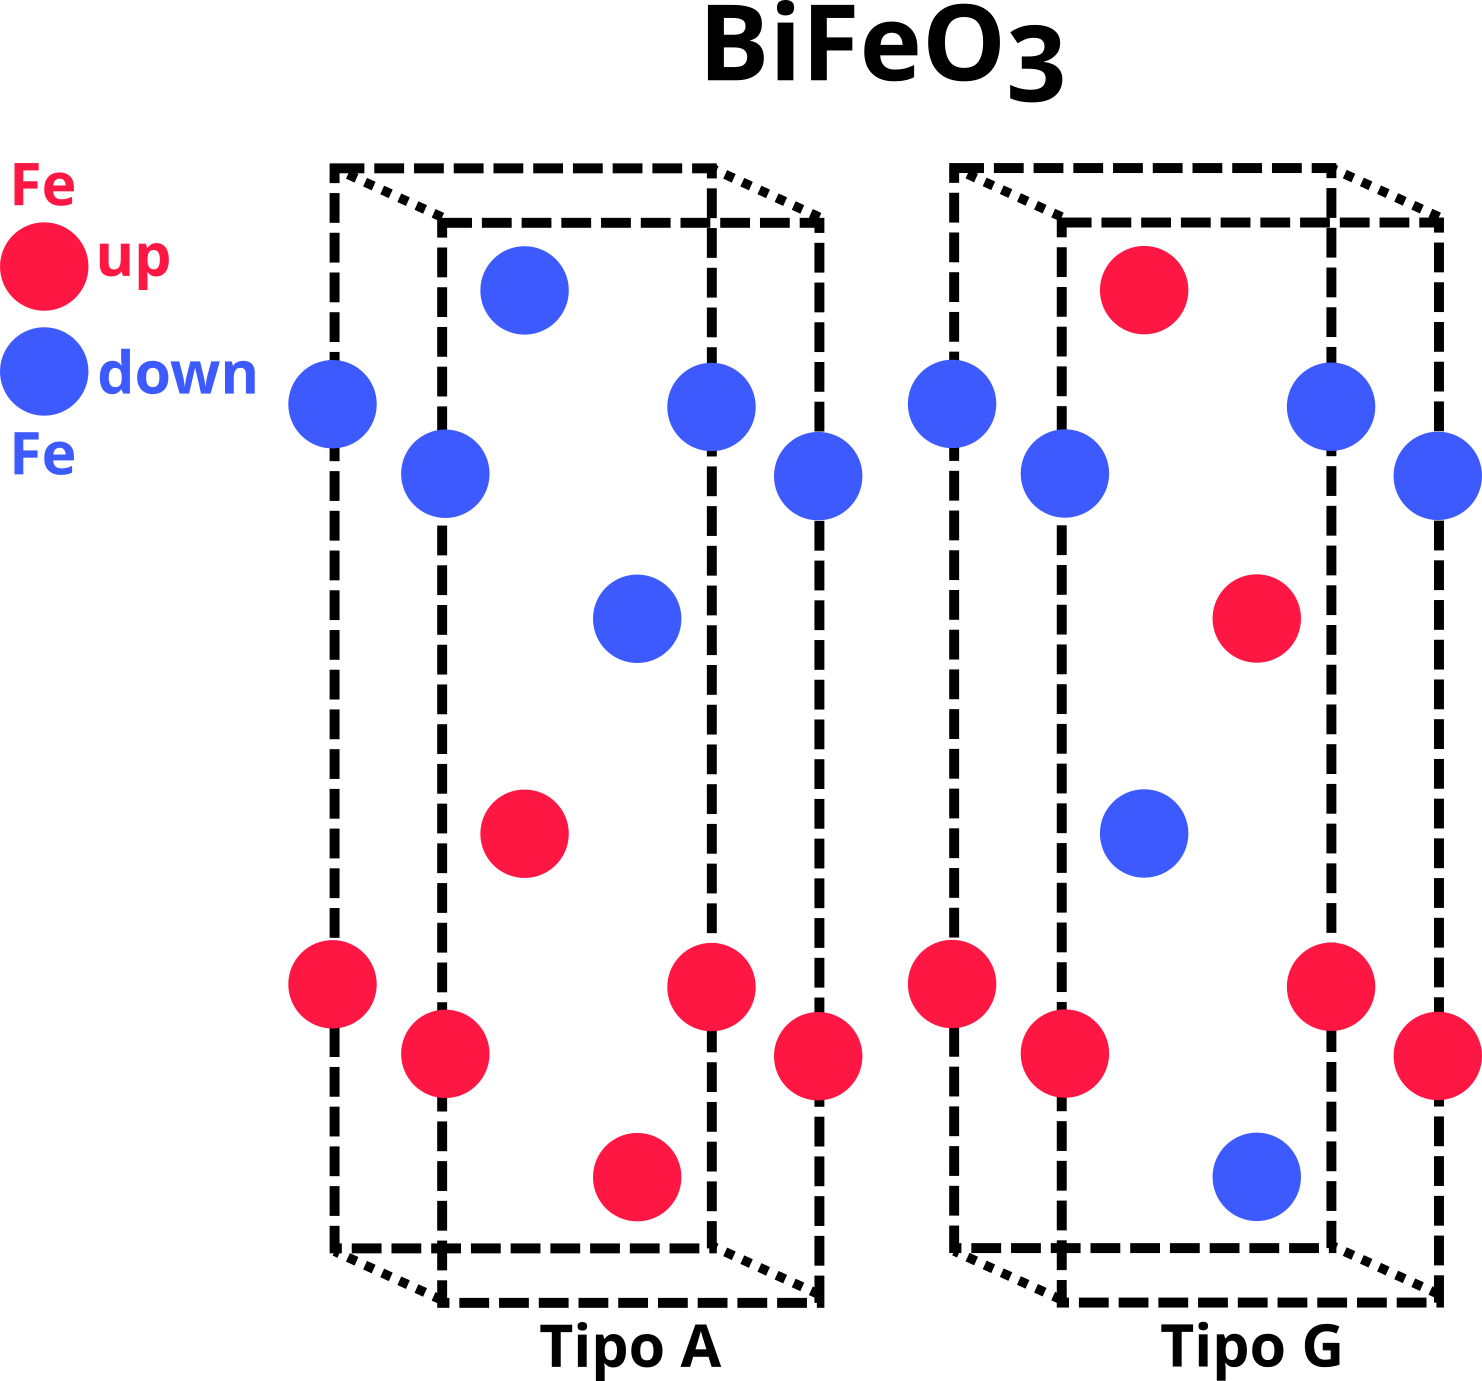
\includegraphics[width=0.5\textwidth]{contenido/calculos_computacionales/arreglos_antiferromagneticos/img_arreglos/BFO_unido.png}
	\caption[Arreglos antiferromagn\'eticos $BiFeO_{3}$]{Arreglos 
		antiferromagn\'eticos para el $BiFeO_{3}$ se muestran solo los \'atomos 
		de hierro por claridad.}
	\label{arreglos_BFO}
\end{figure}

\noindent En el caso del $YCrO_{3}$ se utilizaron los arreglos 
antiferromagn\'eticos tipo 
A, C y G, los cuales se pueden observar en forma esquem\'atica en la figura 
\ref{arreglos_YCO}.

\begin{figure}[H]
	\centering
	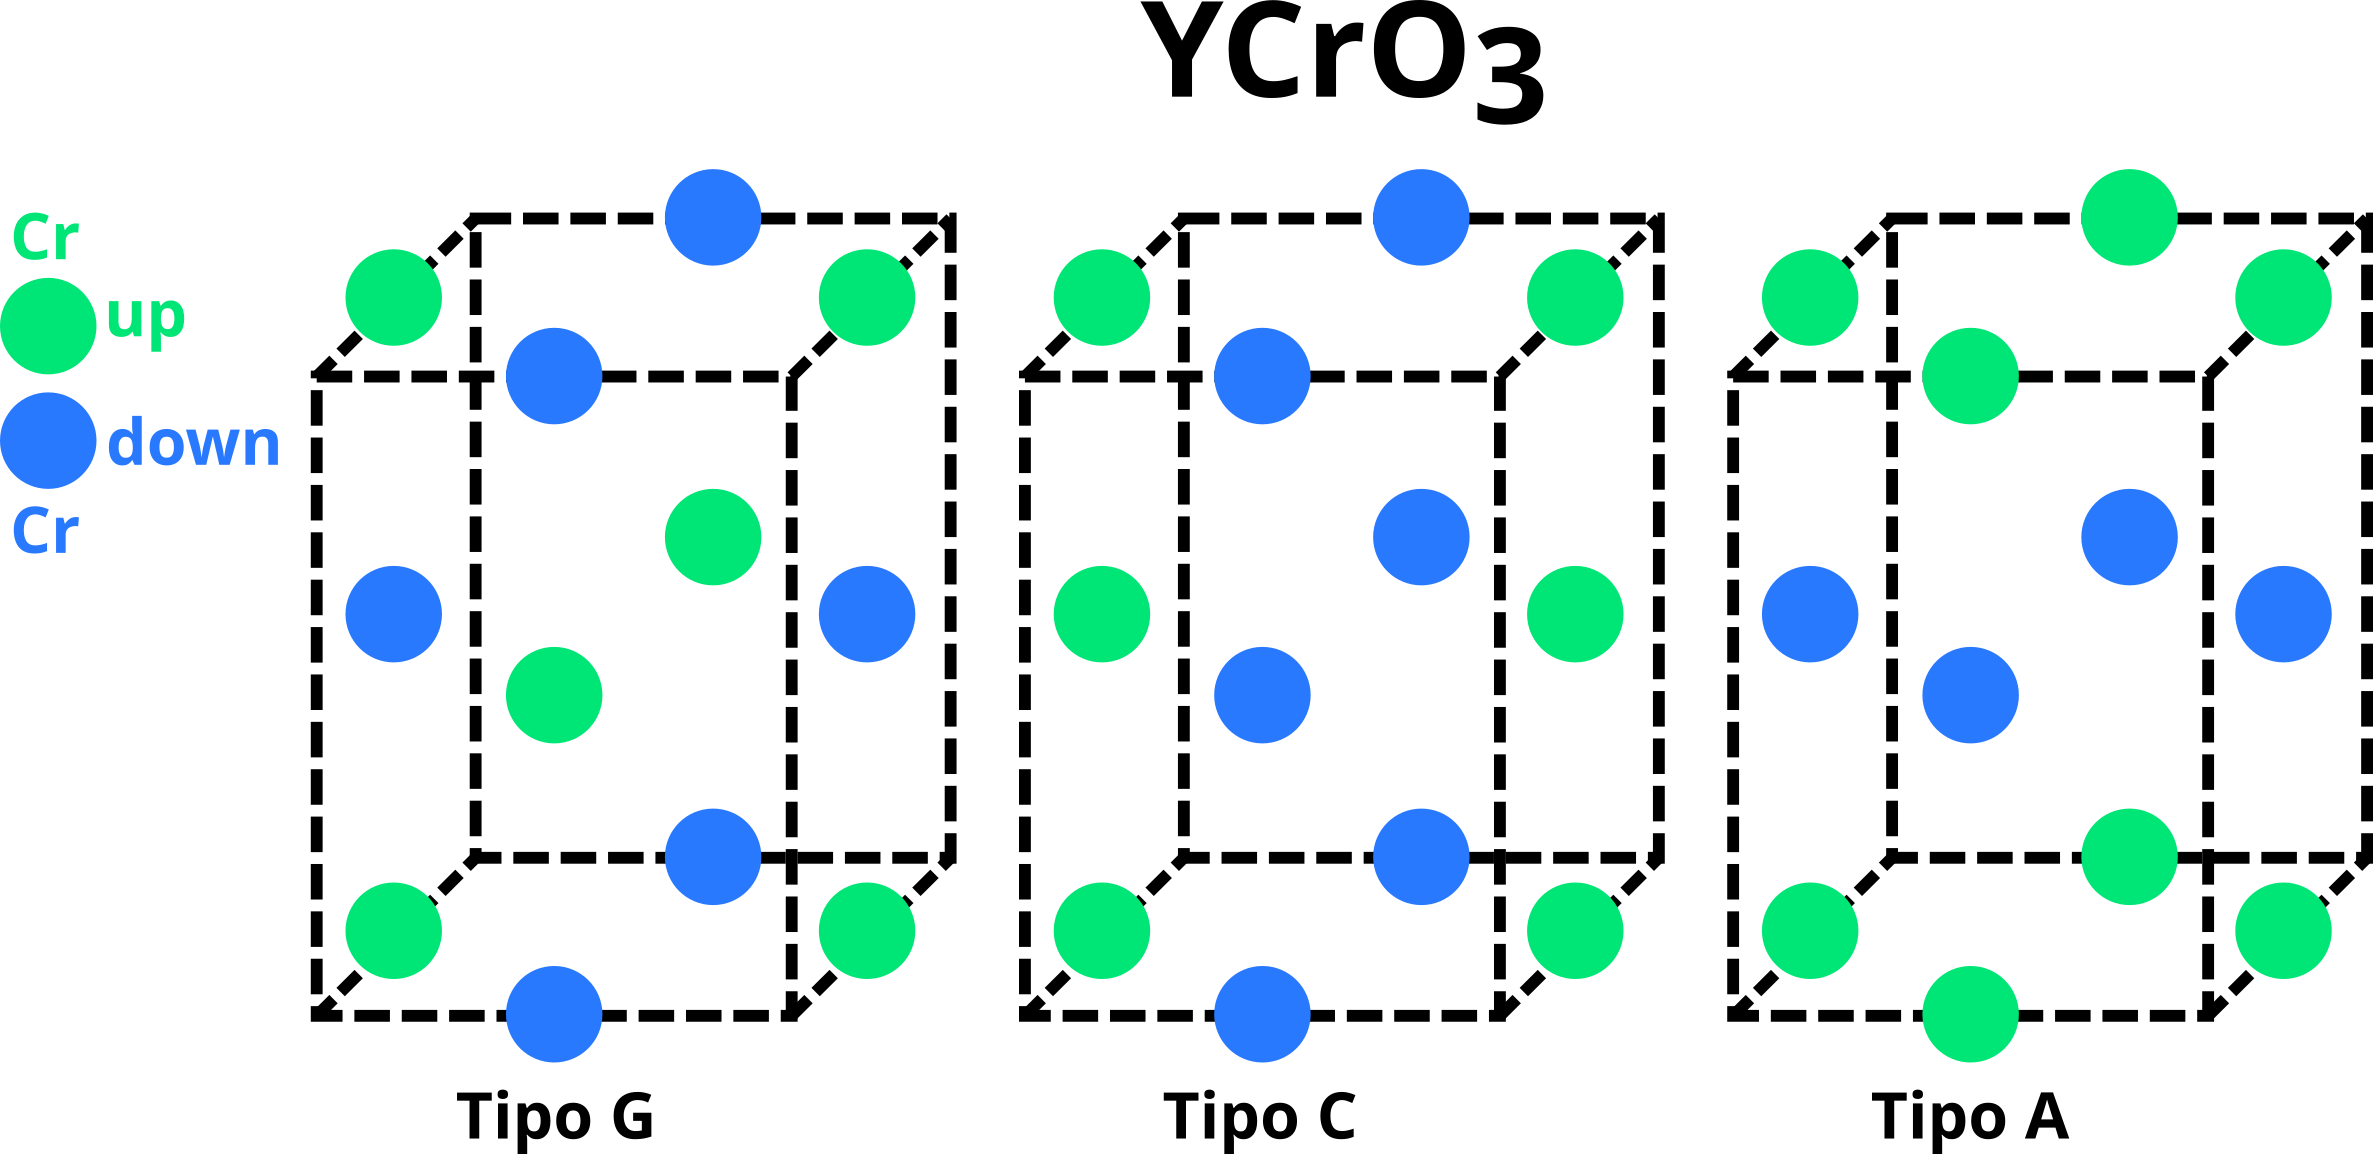
\includegraphics[width=0.6\textwidth]{contenido/calculos_computacionales/arreglos_antiferromagneticos/img_arreglos/YCO_unido.png}
	\caption[Arreglos antiferromagn\'eticos $BiFeO_{3}$]{Arreglos 
		antiferromagn\'eticos para el $YCrO_{3}$ se muestran solo los \'atomos 
		de cromo por claridad.}
	\label{arreglos_YCO}
\end{figure}